\section{Ejercicios}

%\renewcommand{\theenumi}{(\alph{enumi})}

\subsection{Hoja 1}

\subsubsection{Conceptos básicos}

\subsubsection{Algunos métodos de resolución de EDOs}
\textbf{2.18} \begin{enumerate}
	\item $yy'' + {(y')}^2=0$ \\
	      Resulta razonable buscar soluciones en forma de polinomios $y(x)=x^\alpha$ porque:
	      \[\implies y'=\alpha x ^{(\alpha-1)} \we y''=\alpha(\alpha-1)x^{(\alpha-2)}\]
	      \[\implies x^{\alpha}\alpha(\alpha-1)x^{(\alpha-2)} + \alpha^2 x ^{2(\alpha-1)} = 0\implies (2\alpha^2-\alpha)x^\alpha=0\]
	      \[\implies 2\alpha^2-\alpha=0 \implies \alpha(2\alpha-1)=0 \implies \alpha=0 \ve \alpha=\frac{1}{2}\]
	      Opción 1: Integramos la EDO:%\@
	      \[\int_{0}^{t} y(s) y''(s)\odif{s} + \int_{0}^{t} {(y'(s))}^2 \odif{s} = 0\]
	      \[-\int_{0}^t {(y'(s))}^2 \odif{s} + {[y(s)y'(s)]}^t_{s=0} + \int_{0}^{t} {(y'(s))}^2 \odif{s}\]
	      \[\implies y(t)y'(t)-y(0)y'(0)=0 \implies y(t)y'(t)=y(0)y'(0)\eqdef C\]
	      \[\implies \int_{0}^{t} y(s)y'(s)\odif{s}=Ct \implies \frac{{(y(t))}^2}{2}  -\frac{{(y(0))}^2}{2}=Ct\]
	      \[\implies y(t)=\sqrt{2Ct+{(y(0))}^2}\]
	\item $xy''=y'+{(y')}^2$ \\
	      No depende de $y \implies$ Hacemos un cambio de variable $x=y'$:
	      \[\implies xz'=z+z^3 \tex{ que es de variables separadas.}\]
	\item $x^2y''=2xy'+{(y')}^2$ \\
	      Nuevamente hacemos un cambio de variable $z=y' \implies x^2z'=2xz+z^2$
	      \[\forall x \ne 0 : z'=2\frac{z}{x} + {\left(\frac{z}{x}\right)}^2 \implies \tex{ mediante el cambio de variables } \omega = \frac{z}{x}\]
	      Obtenemos una EDO de variables separadas en $\omega$.
	\item $2yy''-{(y')}^2=1$ \\
	      Otra vez resulta razonable buscar soluciones de la forma $y(x)=Ax^2 + Bx +C$
\end{enumerate}

\subsubsection{Modelización}

\textbf{3.4} $C(t)=\tex{``Cantidad de sal''}$ en el tanque en el tiempo $t$.
\[C'(t)=10-\frac{1}{10}C(t) \implies \int_{C(0)}^{C(t)} \frac{1}{100-y}\odif{y} = \int_{0}^{t}\frac{1}{10}\odif{t}\]
\[\implies \log{(100-C(t))} - \log{(100-C(0))}=-\frac{1}{10}\implies \log{\frac{100-C(t)}{100}}=-\frac{t}{10}\]
\[\implies \frac{100-C(t)}{100}=e^{-\frac{t}{10}}\implies C(t)=100(1-e^{-\frac{t}{10}})\]
\[\implies C(1)=100(1-e^{-\frac{1}{10}}) \we \lim_{t\to \infty} C(t) = 100\]

% \textbf{3.7} \begin{enumerate}
% 	\item $xy=C \implies y(x)=\frac{C}{x}$ \\
% 	\begin{enumerate}
% 		\item Sacamos la EDO asociada $\odv{}{x}(xy(x))=\odv{}{x}(C)$
% 		\[\implies y(x) + xy'(x) = 0 \implies y'(x) = -\frac{y(x)}{x}=f(x,y(x))\]
% 		\item Las soluciones de $z'=-\frac{1}{f(x,y(x))}$ son ortogonales a las soluciones de la EDO $y'=f(x,y(x))$.
% 		\item \[z'=-\frac{1}{\frac{z}{x}}=\frac{x}{z} \implies zz'=x \implies \left(\frac{}{}\right)^2\]
% 	\end{enumerate}
% \end{enumerate}
\subsubsection{Análisis cualitativo y campos de pendientes}

\textbf{4.6} $\ds \forall t > \frac{5}{4} : \forall x\left(\frac{5}{4}\right) \in \left(-\sqrt{\frac{5}{4}}, -\frac{1}{2}\right) : x'=x^2-t \implies -\sqrt{t} < x(t) < -\sqrt{t-1}$
\[f_1(t)\defeq-\sqrt{t} \we f_2 \defeq -\sqrt{t-1} \implies f\left(\frac{5}{4}\right)=-\sqrt{\frac{5}{4}} \we f_2\left(\frac{5}{4} - 1\right)=-\frac{1}{2}\]
Sabemos que $\ds \tilde{t} = \frac{5}{4} \implies -\sqrt{\tilde{t}} < x(\tilde{t}) < -\sqrt{\tilde{t}-1}$
\[\implies \tex{Por contunuidad, al menos en un tiempo, estas cotas se siguen manteniendo.}\]
Atendiendo a las isoclinas de este ejercicio $(\{x^2-t=C : C\in \R\})$, observamos que:
\begin{itemize}
	\item $C=0 \implies x^2=t \implies x=\pm\sqrt{t}$ que es precisamente la cota inferior que buscábamos.
	\item $C=-1 \implies x^2-t=-1 \implies x=\pm\sqrt{t-1}$ que es la cota superior.
\end{itemize}
Inicialmente $x(t)>-\sqrt{t}$ ``durante un rato''.
\begin{enumerate}
	\item Supongamos que $\exists t^* : x(t^*)=-\sqrt{t^*}$.
	\item Por un lado, la isoclina nos dice que $x'(t^*)=0$.
	\item Por otro lado, $\ds x'(t^*)\leq {\left[\odv{}{t} (-\sqrt{t})\right]}_{t=t^*} = -\frac{1}{2}\frac{1}{\sqrt{t^*}}<0$.
\end{enumerate}

\textbf{4.7} $\ds \begin{cases}
		x' = x^2 + t^2, t >0 \\
		x(0)>0
	\end{cases}$ Sea $\appl{x}{[0, T)}{\R}$ derivable.
\begin{enumerate}
	\item Queremos ver si $\ds \forall t \in [0, T) : x(t)> \frac{t^3}{3}$ \\
	      Como $\ds x'\geq t^2 \implies \int_{0}^{t} x'(s) \odif{s} \geq \int_{0}^{t} s^2 \odif{s} \implies x(t)-x(0)\geq \frac{t^3}{3}$
	      \[\implies \boxed{\forall t \in [0, T) : x(t)>\frac{t^3}{3}}\]
	\item Queremos ver si $\ds \forall t \in \left(\sqrt{3}, T\right), T>\sqrt{3} : x(t)> \frac{1}{\frac{4}{\sqrt{3}}-t}$ \\
	      Como $\ds x'\geq x^2 \implies x^{-2}x'\geq 1 \implies \int_{\sqrt{3}}^{t} \frac{x'(s)}{{x(s)}^2} \odif{s} \geq t-\sqrt{3}$
	      \[\implies -\frac{1}{x(t)}+ \frac{1}{x(\sqrt{3})} \geq t-\sqrt{3} \implies t \leq \sqrt{3} +\frac{1}{x(\sqrt{3})}- \frac{1}{x(t)}\]
	      \[\implies t< \sqrt{3} + \frac{3}{{\left(\sqrt{3}\right)}^3} - \frac{1}{x(t)}= \sqrt{3} + \frac{1}{\sqrt{3}}- \frac{1}{x(t)}=\frac{4}{\sqrt{3}}- \frac{1}{x(t)}\]
	      \[\implies t < \frac{4}{\sqrt{3}}-\frac{1}{x(t)} \implies \frac{1}{x(t)} < \frac{4}{\sqrt{3}}-t \implies \boxed{\forall t > \sqrt{3} : x(t) > \frac{1}{\frac{4}{\sqrt{3}}-t}}\]
\end{enumerate}

\subsection{Hoja 2}

\textbf{1.1} $\ds \begin{cases}
		x' = f(x) \\
		x(t_0) = x_0
	\end{cases}$ tiene sol única.
\begin{enumerate}
	\item Toda solución que no sea constante es estrictamente monótona.
	      \begin{dem}
		      Por contrarecíproco, veamos que
		      \[\ds \exists t^* : x'(t^*)=0 \implies \forall t : x(t)\equiv C\defeq x(t^*)\]
		      Definimos $\forall t \in \R:y(t)=x(t^*)$. Por hipótesis, $f(C)=f(x(t^*))=x'(t)=0$
		      \[\implies y'(t)=\odv{}{t}(C)=0=f(C)=f(y(t))\implies y \tex{ es solución}\]
		      \[\begin{cases}
				      y'(t)=f(y(t)) \\
				      y(t^*)=C
			      \end{cases} \implies \tex{Por unicidad, } x(t)=y(t)\equiv C\]
	      \end{dem}
	\item $\ds \lim_{t\to \infty} x(t) = C_0 \implies u(t) \equiv C_0$ es solución.
	      \begin{dem}
		      \begin{enumerate}
			      \item $\ds \lim_{t\to \infty} x'(t)=\lim_{t\to \infty}f(x(t)) = f\left(\lim_{t\to \infty} x(t)\right) = f(C_0)$
			      \item Veamos que $f(C_0)=0$. Por contradicción, supongamos que $f(C_0)=A>0$
			            \[\implies \lim_{t\to \infty} x'(t)=A \implies \exists \, \til{t} : \forall t \geq \til{t} : x'(t)>\frac{A}{2}\]
			            \[\implies \int_{\til{t}}^{t} x'(\tau) \odif{\tau} > \int_{\til{t}}^{t} \frac{A}{2} \odif{\tau} \implies x(t)-x\left(\til{t}\right)> \frac{A}{2}(t-\til{t})\]
			            \[\implies \lim_{t\to\infty} x(t) = \lim_{t\to\infty}\left(x\left(\til{t}\right)+\frac{A}{2}\left(t-\til{t}\right)\right)=\infty \contr\]
			      \item $\ds u'(t) = \odv{}{t}(C_0)=0=f(C_0)=f(u(t)) \implies u \tex{ es solución}$.
		      \end{enumerate}
	      \end{dem}
\end{enumerate}

\textbf{1.2} $x'=f(x)$ La unicidad solo se puede perder cuando $f(x)=0$
\begin{enumerate}
	\item $\ds f(x)\defeq x'=\begin{cases}
			      \sqrt{-x} & x<0     \\
			      x^2       & x\geq 0
		      \end{cases}$
	      \begin{obs}\begin{enumerate}
			      \item[]
			      \item $x\equiv 0$ es solución $\left(f(0)=0\right)$ y solo puede haber problemas de unicidad en $x=0$.
			      \item $x(t)$ es estrictamente creciente si $x(t)\ne 0$
		      \end{enumerate}\end{obs}
	      No habría unicidad en $\ds x=0 \iff \lim_{x\to 0} \int_{x}^{x_0} \frac{1}{f(\tau)} \odif{\tau} \in \R$ con $x_0>x$ \\
	      En nuestro caso, $\ds \int_{x}^{x_0} \frac{1}{\tau^2} \odif{\tau} = \frac{1}{x_0} - \frac{1}{x} \xrightarrow{x\to 0^+} -\infty \implies \tex{ hay unicidad por arriba.}$ \\
	      Para la unicidad por abajo, $\ds \int_{x_0}^{x} \frac{1}{\sqrt{-\tau}} \odif{\tau} = -2\left(\sqrt{-x} - \sqrt{-x_0}\right) \xrightarrow{x\to 0^-} 2 \sqrt{x_0} \in \R$
	      \[\implies \tex{No hay unicidad por abajo.}\]
	      Por tanto, podemos encontrar una solución de la siguiente forma:
	      \[y(t)\defeq \begin{cases}
			      -\frac{t^2}{4} & t<0     \\
			      0              & t\geq 0
		      \end{cases} \implies y'(t)=\begin{cases}
			      -\frac{t}{2} & t<0     \\
			      0            & t\geq 0
		      \end{cases}\]
	      Es solución porque:
	      \[f(y(t))=\begin{cases}
			      f(-\frac{t^2}{4}) & t<0     \\
			      f(0)              & t\geq 0
		      \end{cases} = \begin{cases}
			      \sqrt{-\left(-\frac{t^2}{4}\right)} & t<0     \\
			      0                                   & t\geq 0
		      \end{cases} = \begin{cases}
			      -\frac{t}{2} & t<0     \\
			      0            & t\geq 0
		      \end{cases} = y'(t)\]
	      Por un lado, $\ds x(t_0)=0 \implies \lim_{t\to \infty}x(t)=0 \tex{ por la unicidad por arriba.}$ \\
	      Por otro lado, si $x(t_0)<0$ sabemos que
	      \begin{itemize}
		      \item $x(t)$ no decrece.
		      \item $x(t)$ está acotada por arriba por 0.
	      \end{itemize}
	      \[\implies \exists \lim_{t\to \infty} x(t) \leq 0\]
	      Supongamos que $\ds \exists A > 0 : \lim_{x(t)} = -A$. \\
	      Como $x(t)$ no decrece,
	      \[\ds \implies x(t) \leq -A \implies x'(t) = \sqrt{-x(t)}\geq \sqrt{A} \implies x(t)\geq x(c) + \sqrt{A}t \xrightarrow{t\to \infty} \infty \contr\]
	      \[\implies \lim_{t\to \infty} x(t) =0 \]
	\item
\end{enumerate}

\textbf{1.3} $\ds x' = f(t,x) \we x$ es solución.
\[f\tex{ no depende de } t \iff \forall b \in \R : y(t)\defeq x(t+b) \tex{ es sol.}\]
\begin{dem}
	$(\implies)$ Supongamos que $f$ no depende de $t$.
	\[\implies x'=f(x) \implies y(t)=x(t+b)\implies y'(t)=\odv{}{t} (x(t+b)) = x'(t+b)\]
	\[\implies y'(t)=f(x(t+b))=f(y(t))\]
	$(\impliedby)$ Supongamos que $\forall b \in \R : y(t)\defeq x(t+b) \tex{ es sol.}$
	\[x'=f(t, x(t)) \implies y(t)=x(t+b) \tex{ también es solución}\]
	\[x'(t+b)=f(t, x(t+b)) \implies x'(t) = f(t-b, x(t))\]
	\[\implies \forall b \in \R : f(t-b, x(t))=f(t, x(t))\]
	En particular, $x(0)=x_0 \in \R \implies \forall b \in \R : \forall x_0 \in \R : f(-b,x_0)=f(0,x_0)$
	\[\implies f\tex{ no depende de su primera variable}\]
\end{dem}

\subsection{Hoja 3}
\textbf{1.3} \[ \begin{cases} x' = t+x \\ x(0)=1\end{cases} \iff x(t) = 1 +\frac{t^2}{2} + \int_{0}^{t} x(s) \odif{s} \eqdef T[x](t)\]
Definimos la sucesión de funciones $x_{n+1}(t) = T[x_n](t) \we x_1(t) = x(0) = 1$ y tenemos:
\[\begin{aligned}
		x_2(t) & = T[x_1](t) = 1 + \frac{t^2}{2} + \int_{0}^{t} 1 \odif{s} = 1 + \frac{t^2}{2} + t                                                                                   \\
		x_3(t) & = T[x_2](t) = 1 + \frac{t^2}{2} + \int_{0}^{t} \left(1 + \frac{s^2}{2} + s \right) \odif{s} = 1 + \frac{t^2}{2} + t + \frac{t^3}{6} + \frac{t^2}{2}                 \\
		\vdots                                                                                                                                                                       \\
		x_n(t) & = 1 + t + 2 \sum_{j=2}^{n-1} \frac{t^j}{j!} + \frac{t^n}{n!} = -1 - t + 2 \sum_{j=0}^{n} \frac{t^j}{j!} - \frac{t^{n}}{n!} \xrightarrow{n \to \infty} -1 -t +2e^t+0
	\end{aligned}\]
\[\implies \boxed{x(t) = -1-t+2e^t}\]

\textbf{2.1}
\begin{enumerate}
	\item $f_n(x) = x^{\sfrac{1}{n}}$ en $x\in [0,1]$
	      \[f_n(0)=0 \implies \lim_{n\to \infty} f_n(0) = 0 \quad \we \quad x_0 \in (0, 1] \implies \lim_{n\to \infty} x_0^{\sfrac{1}{n}} = 1\]
	      \[\implies f_n \xrightarrow{n\to\infty} f \tex{ puntualmente en } [0, 1] \tex{ con } f(x)= \begin{cases} 0 & x=0 \\ 1 & x\in (0, 1] \end{cases}\]
	      ¿Converge uniformemente? Sabemos $\forall n : f_n \tex{ cont.} \we f_n\rightarrow f \text{ unif.} \implies f \tex{ cont}$. \\
	      Como $f$ no es continua $\implies f_n$ no converge uniformemente.
	\item $f_n(x) = \frac{nx}{1+nx}$ en $x\in [0,\infty)$
	      \[f_n(0)=0 \implies \lim_{n\to \infty} f_n(0) = 0 \quad \we \quad \forall x_0 > 0 : \lim_{n\to \infty} \frac{nx_0}{1+nx_0} = 0\]

\end{enumerate}
\begin{obs}
	\begin{enumerate}
		\item[]
		\item $\ds f_n \xrightarrow{n\to \infty} f \tex{ puntualmente en } \Omega \iff \forall x \in \Omega : \lim_{n\to \infty} f_n(x) = f(x)$
		      \[\iff \forall x \in \Omega : \forall \varepsilon > 0 : \exists n_0(x) \in \N : \forall n > n_0(x) : \abs{f_n(x)-f(x)}<\varepsilon\]
		\item $\ds f_n \xrightarrow{n\to \infty} f \tex{ uniformemente en }\Omega\iff \sup_{x\in \Omega} \abs{f_n(x)-f(x)} \xrightarrow{n\to \infty} 0$
		      \[\iff \forall \varepsilon > 0 : \exists n_0 \in \N : \forall n > n_0 : \forall x \in \Omega : \abs{f_n(x)-f(x)}<\varepsilon\]
	\end{enumerate}
\end{obs}

\textbf{2.2} Estudiamos la sucesión de funciones en $f_n(x)=n^2xe^{-nx^2} $ en $x\in [0,1]$
\begin{enumerate}
	\item Convergencia puntual: $\ds \forall n \in \N : f_n(0) \implies \lim_{n\to\infty} f_n(0) = 0$
	      \[x_0 \in (0, 1] \implies \lim_{n\to \infty} n^2x_0e^{-nx_0^2} = 0 \implies f_n\xrightarrow{n\to \infty} 0 = f \tex{ puntualmente en } [0,1]\]
	\item Convergencia uniforme: $\ds \sup_{x\in [0,1]} \abs{f_n(x)-f(x)} = \sup_{x\in [0,1]} \abs{f_n(x)-0} = \sup_{x\in [0,1]} n^2xe^{-nx^2}$
	      \[f_n'(x) = n^2e^{-nx^2} - 2n^3x^2e^{-nx^2} = n^2e^{-nx^2}(1-2nx^2) \implies f_n'(x)=0 \iff x=\frac{1}{\sqrt{2n}}\]
	      \[\frac{1}{\sqrt{2n}} \in [0, 1] \implies \sup_{x\in[0, 1]} \abs{f_n(x)} = f_n\left(\frac{1}{\sqrt{2}n}\right) = \frac{n^{\sfrac{5}{2}}}{\sqrt{2}}e^{-\frac{1}{2}} \xrightarrow{n\to\infty} \infty\]
	      Por tanto, $f$ no converge uniformemente.
	\item \textbf{Nota:} Cuando falla la convergencia uniforme, el límite de la integral no es necesariamente igual a la integral del límite.
	      \[\ds \lim_{n\to\infty} \int_{0}^{1} f_n(x) \odif{x} = \infty \ne 0 = \lim_{n\to\infty} 0 = \int_{0}^{1} 0 \odif{x} = \int_{0}^{1} f(x) \odif{x}\]
\end{enumerate}

\begin{obs}
	\begin{enumerate}
		\item[]
		\item $\ds f \tex{ es Lipschitz en } \Omega \iff \exists L \geq 0 : \forall x, y \in \Omega : \abs{f(x)-f(y)}\leq L\abs{x-y}$
		\item $\ds f \tex{ es localmente Lipschitz en } \Omega \iff \forall K \subset \Omega \tex{ compacto} : f \tex{ es Lipschitz en } K$
	\end{enumerate}
\end{obs}

\fecha{05/04/2024}

\textbf{Prolongabilidad de soluciones:}
Si hay existencia y unicidad local para $(x_0, y_0)\in D$, entonces la solución solo puede dejar de existir si ``explota'' en $D$. Por ejemplo:
\[\begin{cases}
		y' = y^2 \\
		y(x_0) = y_0
	\end{cases} \xRightarrow{\tex{P-L}} \forall (x_0, y_0) \in \R\times\R : \exists ! \tex{ solución en un entorno de } (x_0, y_0)\]

\textbf{4.1} a) $\ds y' = \frac{xy + y^2}{x^2 + y^2 + 2} \eqdef f(x, y)$
\[f\in \mathcal{C}^1(\R^2) \implies \forall (x_0, y_0) \in \R^2 : \exists ! \tex{ solución local }\]
\[y(x)=0 \tex{ es solución de la EDO }\implies \begin{cases}
		y_0>0 \implies \forall x \in \R : y(x)>0 \\
		y_0=0 \implies \forall x \in \R : y(x)=0 \\
		y_0<0 \implies \forall x \in \R : y(x)<0 \\
	\end{cases}\]

Queremos una función $\appl{g}{\R}{\R} : y(x) \leq g(x)$.
\begin{itemize}
	\item Supongamos por un momento que $\abs{f(x, y)}\leq K$.
	      \[\ds \begin{aligned}
			      y(x)=y(x_0) + \int_{x_0}^x f(s, y(s)) \odif{s}\implies
			      \abs{y(x)} & \leq \abs{y(x_0)} + \int \abs{f(s,y(s))} \odif{s} \\
			                 & \leq \abs{y(x_0)} + K\abs{x-x_0}
		      \end{aligned}\]
	      \[\implies \forall x \in \R : 0 < y(x) \leq \abs{y(x_0)} + K\abs{x-x_0} \eqdef g(x)\]
	      \[\exists K \in \R : \abs{f(x, y)} \leq K \implies y(x) \tex{ existe para (y desde) siempre}\]

	\item Por tanto, basta ver que $f(x, y) \leq 2$
	      \[\abs{f(x, y)} \leq \frac{\abs{x} \abs{y} + y^2}{x^2+y^2 +2}\leq \frac{x^2+y^2 + y^2}{x^2+y^2 +2} \leq \frac{x^2 + y^2}{x^2+y^2+2}\leq 2\]
\end{itemize}

b) $\ds \left\{x'=\frac{x^2+t^4}{\sqrt{1+x^2+t^2}} \we x(t_0) = x_0\right\}$ $f\in \mathcal{C}^1(\R^2) \implies \forall (x_0, t_0) \in \R^2 : \exists ! \tex{ solución local}$
\[\forall (t, x) \in \R^2 : f(t, x) \geq 0 \implies x'(t) \geq 0 \implies \begin{cases}
		\forall t \geq t_0 : x(t) \geq x_0 \\
		\forall t \leq t_0 : x(t) \leq x_0
	\end{cases}\]

\[\abs{f(t, x)} = f(t, x) = \frac{x^2}{\sqrt{1+x^2+t^2}} + \frac{t^4}{\sqrt{1+x^2+t^2}} \leq \frac{x^2}{\abs{x}} + \frac{t^4}{\abs{t}} \leq \abs{x} + \abs{t^3}\]

Tomamos $T>0$ arbitrario y demuestro que la solución existe para todo $t\in [t_0-T, t_0+T]$. Usamos la forma integral para acotar:
\[\begin{aligned}
		\abs{x(t)} & \leq \abs{x(t_0)} + \int_{t_0}^{t} \abs{f(s, x(s))} \odif{s} \leq \abs{x(t_0)} + \int_{m\defeq \min\{t, t_0\}}^{M\defeq \max\{t, t_0\}} \abs{f(s, x(s))} \odif{s} \\
		           & \leq \abs{x(t_0)} + \int_{m}^{M} \abs{x(s)} + \abs{s^3} \odif{s}                                                                                                  \\
		           & = \abs{x(t_0)} + \left(\max\{\abs{t_0-T}, \abs{t_0+T}\}\right)^3\abs{t-t_0} + \int_{m}^{M} \abs{x(s)} \odif{s}                                                    \\
		           & \leq C(x_0, t_0, T) + \int_{m}^{M} \abs{x(s)} \odif{s} \xRightarrow{\tex{Gronwall}} \abs{x(t)} \leq Ce^{t-t_0}
	\end{aligned}\]

\begin{lem}[Gronwall]
	Sea $\appl{g}{[a, b]}{\R}$ continua y $C\geq 0$ tal que \\
	$\ds \forall t \in [a, b] : g(t) \leq C + \int_{a}^{b} g(s) \odif{s}\implies \forall t \in (a, b) : g(t) \leq Ce^{b-a}$
	\begin{dem}
		Definimos $\ds G(t) \defeq C + \int_a^b g(s) \odif{s}\implies G(t_0) = C \we G'(t) = g(t) $
		\[\implies \begin{cases}
				G'(t) \leq G(t) \\
				G(t_0) = C
			\end{cases}\implies G(t) \leq C e^{t-t_0} \implies g(t) \leq C e^{t-t_0}\]
	\end{dem}
\end{lem}

\textbf{4.3} $\ds x'=x^5 + \frac{tx^2}{1+x^2} \eqdef f(t,x)$
\[\tex{a) } \quad f\in \mathcal{C}^1(\R^2) \implies \forall (t_0, x_0) \in \R^2 : \exists ! \tex{ solución local}\]
\[\tex{b) } \quad x(0) = x_0 > 0 \implies \forall t \leq 0 : \tex{La solución se puede definir}\]
\[\forall t \in \R : \underline{x}(t) \defeq 0 \tex{ es solución} \implies \forall t \in \R : x(t) > 0 \tex{ (mientras exista)}\]

Quiero acotar $\abs{f(t, x)}$ por debajo de $x$.
\[x' = x^5 + \frac{tx^2}{1+x^2} \geq t\frac{x^2}{1+x^2} \geq t\implies \int_t^0 x'(s) \odif{s} \geq \int_t^0 s \odif{s} \implies x(t) \leq x(0)+ \frac{t^2}{2}\]
\[\tex{c) } \quad x(0) = x_0 > 0 \implies \tex{La solución no existe despues de un }T_+\]
\[x'= x^5 + \frac{tx^2}{1+x^2} \geq x^5 \implies \cdots \implies 4(x(t))^4 \geq \frac{1}{\frac{1}{4x_0^4} - t} \implies \boxed{T_+ = \frac{1}{4x_0^4}}\]

\textbf{4.4} $\lambda > 0 \we \begin{cases}
		y' = y^4 + \lambda \\
		y(0) = y_0
	\end{cases}$

\[\tex{a) } \quad \begin{cases}
		y'\geq y^4 \\
		y(c) = c
	\end{cases} \implies \xcancel{T_+=\frac{1}{3x_0}}\]

\textbf{5.3} (Variado) $\ds \left\{x'=\frac{2}{1+t^2} \cos{\left(x+ \frac{\pi}{2}\right)} \we x_1(0)=a  \we x_2(0)=b\right\}$ con $0 < a < b$.

\begin{enumerate}
	\item $x \equiv 0$ es solución de la EDO.
	\item $f$ es Lipschitz en $x$, uniformemente en $t \implies \forall (t_0, x_0) \in \R^2 : \exists ! \tex{ solución global}$
	\item $x_1(0) = a \we x_2(0) = b \implies \forall t \in \R : x_1(t) , x_2(t) > 0$.
	\item $0<a<b<\pi \implies \bar{x}(t)=\pi$ es solución $\implies 0<x_1(t), x_2(t)<\pi$.
	\item Como no se pueden cortar porque se perdería unicidad, $\forall t \in \R : x_1(t) < x_2(t)$.
\end{enumerate}
\[i = 1,2 : x_i(t) = x_i(0) + \int_{0}^{t} \frac{2}{1+s^2} \cos{\left(x_i(s)+\frac{\pi}{2}\right)} \odif{s}\]
\[\implies x_2(t) - x_1(t) =x_2(0) - x_1(0) + \int_{0}^{t} \frac{2}{1+s^2} \left(\cos{\left(x_2(s)+\frac{\pi}{2}\right)} - \cos{\left(x_1(s)+\frac{\pi}{2}\right)}\right) \odif{s}\]
\[\implies \abs{x_1(t) - x_2(t)} \leq \abs{a-b} + \int_{0}^{t} \underbrace{\frac{2}{1+s^2}}_{\leq 2} \underbrace{\abs{\cos{\left(x_2(s)+\frac{\pi}{2}\right)} - \cos{\left(x_1(s)+\frac{\pi}{2}\right)}}}_{\leq \abs{x_1(s) - x_2(s)}} \odif{s}\]
\[z(t) \defeq \abs{x_1(t) - x_2(t)} \implies z(t) \leq (b-a) + 2\int_{0}^{t} z(s)\odif{s} \eqdef G(t)\]
\[\implies G'(t) = 2 z(t) \leq 2 G(t) \implies \begin{cases}
		G'(t) \leq 2 G(t) \\
		G(0) = b-a
	\end{cases} \implies G'(t) - 2G(t) \leq 0\]
\[\left(G'(t) - 2G(t)\right) e^{-2t} = \left(G(t)e^{-2t}\right)' \leq 0 \implies G(t)e^{-2t} - G(0) e^{-2\cdot 0} \leq 0\]
\[\implies G(t) \leq (b-a)e^{2t} \implies z(t) \leq (b-a)e^{2t} \implies \forall t > 0 : \abs{x_1(t) - x_2(t)} \leq (b-a) e^{2t}\]
Sea $\left(a_k\right): a_k \xrightarrow{k\to \infty} b$ y definimos $x_k$ la solución del PVI cuando $x_k(0)=a_k$.\\
Entonces, la sucesión de funciones $\left(x_k\right)$ converge uniformemente a $x_2$.

\textbf{5.2} $\ds x' = x + \sin(tx) \we y' = \sin(ty) \we x(0) = y(0) = 1$ (Cae siempre en el examen).
\begin{enumerate}
	\item $\exists ! \tex{ solución global para ambas}$
	\item $x(t), y(t) > 0$ (0 es solución de ambas EDOs).
	\item $\forall t > 0 : x(t) > y(t)$
	      \begin{dem}
		      Vemos que $x(0)=y(0) = 1 \we x'(0) = 1 \we y(0) = 0$.

		      Suponemos que $\exists t^* : x(t^*) = y(t^*)$, sabemos que $x(t) > y(t)$ para $t\in(0, t^*)$
		      \[\implies y'(t^*) \geq x'(t^*)\]
		      Por otro lado, $x'(t^*) = x(t^*) + \sin(t^*x(t^*)) > \sin(t^*y(t^*)) = y'(t^*) \contr$
	      \end{dem}
\end{enumerate}
Escribimos las soluciones integrales, las restamos y aplicamos la desigualdad triangular.
\[\implies x(t) - y(t) = \cancelto{0}{x(0) - y(0)} + \int_{0}^{t} \left(\sin(sx(s)) - \sin(sy(s))\right) \odif{s} + \int_{0}^{t} x(s)\odif{s}\]
\[\implies \abs{x(t) - y(t)} \leq \int_{0}^{t} s \abs{x(s) - y(s)} \odif{s} + \int_{0}^{t} \abs{x(s)} \odif{s}\]
Queremos encontrar una barrera para $x$, i.e. una función $f$ tal que $x(t) \leq f(t)$.
\[\forall a \in \R : \sin{a} \leq a \implies x'(t) = x(t) + \sin{(tx)} \leq x(t) + tx = (1+t)x(t)\]
\[\implies x'-(1+t)x \leq 0 \implies e^{-t-\frac{t^2}{2}}\left(x'-(1+t)x\right) = \left(x(t)e^{-t-\frac{t^2}{2}}\right)'\leq 0\]
\[\implies x(t)e^{-t-\frac{t^2}{2}} -1 \leq 0 \implies 0 \leq x(t) \leq e^{t+\frac{t^2}{2}} \eqdef f(t)\]
\[z(t) \defeq \abs{x(t) - y(t)} \implies z(t) \leq \int_{0}^{t} s z(s) \odif{s} + \int_{0}^{t} f(s) \odif{s} \eqdef G(t)\]
\[\implies G'(t) = tz(t) +f(t) \leq tG(t) + f(t) \implies \begin{cases}
		G'(t) \leq tG(t) + f(t) \\
		G(0) = 0
	\end{cases}\]
\[\implies e^{-\frac{t^2}{2}}\left(G'(t) - tG(t)\right) \leq f(t) e^{-\frac{t^2}{2}} \implies \left(G(t) e^{-\frac{t^2}{2}}\right)' \leq e^{t}\]
\[\implies \cdots \implies \forall t > 0 : z(t)\leq G(t) \leq e^{\frac{t^2}{2}}\left(e^t -1 \right)\]
¿Y para tiempos negativos $(t < 0)$? Definimos $\bar{x}(t) \defeq x(-t) \we \bar{y}(t) \defeq y(-t)$.

\textbf{6.4} $\ds x' = {\left(\sin\left(\frac{\sqrt{x-t^2}}{t}\right)\right)}^2 = f(t, x)$

a) Existencia y unicidad. Sea $\mathcal{A} = \{(t, x) \in \R^2 : x \geq t^2 \we t\ne 0\}$. ¿Es Lipschitz?
\[t > 0 \implies \abs{f(t, x) - f(t, y)} = \abs{ \pdv{f}{x} (t, \xi)}\abs{x-y}\]
\[\pdv{f}{x}(t,x) = 2\sin\left(\frac{\sqrt{x-t^2}}{t}\right)\cos\left(\frac{\sqrt{x-t^2}}{t}\right)\frac{1}{2t\sqrt{x-t^2}}\]
\[\implies \abs{\pdv{f}{x}(t,x )} \leq 2 \frac{\cancel{\sqrt{x-t^2}}}{t} \cdot 1 \cdot \frac{1}{2t\cancel{\sqrt{x-t^2}}} = \frac{1}{t^2}\]
Por tanto, hay existencia y unicidad local en $\mathcal{A}$.

b) Definimos el problema de valores iniciales con $x(1) = 3$.
\begin{enumerate}
	\item $x(t) \geq 3$ porque $x'(t) \geq 0 \implies x(t) \geq x(1) = 3$.
	\item $\ds x(t) \leq 2 + t$ porque $\ds \abs{x(t)} \leq \abs{x(1)} + \int_{1}^{t} \underbrace{\abs{f(s, x(s))}}_{\leq 1} \odif{s} \leq 3 + (t-1) = t+2$.
\end{enumerate}

\subsection{Hoja 4}

\subsubsection{Sistemas lineales de primer orden}

\textbf{1.1} $\ds \vec{X}'(t) = \begin{pmatrix} 1 & 3 \\ 3 & 1 \end{pmatrix} \vec{X}(t) \we \vec{X}(0) = \begin{pmatrix} 5 \\ 1 \end{pmatrix}$

Supongamos que tenemos $\vec{v} \in \R^2 : A\vec{v} = \lambda \vec{v}$, definimos $\vec{u} \defeq e^{\lambda t} \vec{v}$.
\[\implies \vec{u}'(t) = \lambda e^{\lambda t} \vec{v} = e^{\lambda t} (\lambda \vec{v}) = e^{\lambda t} (A \vec{v}) = A e^{\lambda t} \vec{v} = A \vec{u}(t) \implies \vec{u} \tex{ es una solución del SLH}\]
\begin{enumerate}
	\item Por tanto, encontrar autovalores y autovectores de $A\implies $encontrar soluciones.
	\item El espacio vectorial de soluciones es de dimensión 2.
	\item Dos soluciones linealmente independientes generan todas las soluciones.
\end{enumerate}
\[\det(A-\lambda I ) = 0 \implies \begin{vmatrix} 1-\lambda & 3 \\ 3 & 1-\lambda \end{vmatrix} = 0 \implies \lambda^2 - 2\lambda - 8 = 0 \implies \lambda_1 = 4 \we \lambda_2 = -2\]
\begin{itemize}
	\item $\lambda_1 = 4 \implies \begin{pmatrix} -3 & 3 \\ 3 & -3 \end{pmatrix} \begin{pmatrix} v_1^1 \\ v_1^2 \end{pmatrix} = \begin{pmatrix} 0 \\ 0 \end{pmatrix} \implies v_1^1 = v_1^2 \implies \vec{v_1} = \begin{pmatrix} 1 \\ 1 \end{pmatrix}$
	\item $\lambda_2 = -2 \implies \begin{pmatrix} 3 & 3 \\ 3 & 3 \end{pmatrix} \begin{pmatrix} v_2^1 \\ v_2^2 \end{pmatrix} = \begin{pmatrix} 0 \\ 0 \end{pmatrix} \implies v_2^1 = -v_2^2 \implies \vec{v_2} = \begin{pmatrix} 1 \\ -1 \end{pmatrix}$
\end{itemize}
\[\implies \tex{la solución general del SLH es }\vec{X}(t) = c_1 e^{4t} \begin{pmatrix} 1 \\ 1 \end{pmatrix} + c_2 e^{-2t} \begin{pmatrix} 1 \\ -1 \end{pmatrix}\]
\[\begin{pmatrix} 5 \\ 1 \end{pmatrix} = \vec{X}(0) = c_1 \begin{pmatrix} 1 \\ 1 \end{pmatrix} + c_2 \begin{pmatrix} 1 \\ -1 \end{pmatrix} \implies \begin{cases}
		c_1 + c_2 = 5 \\
		c_1 - c_2 = 1
	\end{cases} \implies c_1 = 3 \we c_2 = 2\]
\[\implies \tex{la solución del PVI es }\vec{X}(t) = 3 e^{4t} \begin{pmatrix} 1 \\ 1 \end{pmatrix} + 2 e^{-2t} \begin{pmatrix} 1 \\ -1 \end{pmatrix}\]

\textbf{1.5} b) Vemos que $W(f_1(t), f_2(t)) = 0$. Viendo las implicaciones anteriores, concluimos que $f_1(t)$ y $f_2(t)$ no son soluciones de una EDO con unicidad.

\subsubsection{EDO lineales de orden superior}

\textbf{2.11} Sea $y'' +y = 0$ una EDO de segundo orden. Definimos $z\defeq y' \implies z' = y''= -y$.\\
Por tanto, tenemos el sistema de EDOs de primer orden:
\[\begin{pmatrix}
		y' \\
		z'
	\end{pmatrix} = \begin{pmatrix}
		0  & 1 \\
		-1 & 0
	\end{pmatrix} \begin{pmatrix}
		y \\
		z
	\end{pmatrix} \implies \tex{autovalores } \lambda = \pm i\]
Veamos que $\mathcal{B} = \left\{ b_1(x) = \cos(x) - \sin(x), b_2(x) = 2\sin(x) \right\}$ es una base de soluciones.

Como $\cos{x}, \sin{x}$ son soluciones de la ecuación y $b_1, b_2$ son combinaciones lineales de $\cos{x}, \sin{x}$, entonces son soluciones.
Una manera: \[\forall x \in \R : a_1(\cos(x) - \sin(x)) + a_2 2 \sin(x) = 0 \implies \begin{cases}
		x= 0 \implies a_1 = 0 \\
		x= \frac{\pi}{2} \implies a_2 = 0
	\end{cases}\implies \tex{l.i.}\]
Otra manera:
\[\forall x \in \R : \begin{cases}
		a_1b_1(x) + a_2b_2(x) = 0 \\
		a_1b_1'(x) + a_2b_2'(x) = 0
	\end{cases} \iff \begin{pmatrix}
		b_1  & b_2  \\
		b_1' & b_2'
	\end{pmatrix} \begin{pmatrix}
		a_1 \\
		a_2
	\end{pmatrix} = 0\]
Si $\exists x \in \R : \det \neq 0 \implies a_1 = a_2 = 0$ es la única solución.
\[\begin{vmatrix}
		\cos(x) - \sin(x)  & 2\sin(x) \\
		-\sin(x) - \cos(x) & 2\cos(x)
	\end{vmatrix} = \cdots = 2\cos^2(x) + 2\sin^2(x) = 2 \neq 0 \implies \tex{l.i.}\]
\textbf{Obs:} no sólo $\exists x\in \R : \det \neq 0$ sino que $\forall x \in \R : \det \neq 0$. ¿Coincidencia? NO.

\textbf{Importante:} Sean $b_1, b_2$ soluciones de la EDO con unicidad.
\[\exists x \in \R : W(b_1(x), b_2(x)) \neq 0 \iff \forall x \in \R : W(b_1(x), b_2(x)) \neq 0 \iff b_1, b_2 \tex{ l.i.}\]

Sea $x^2y'' - 4xy'+(x^2+6)y = 0$ una EDO de segundo orden. Si además $y(0) = y'(0) = 0$ tenemos que $y_1(x)=x^2\sin{x} \we y_2(x)= 0$ son soluciones de la EDO. Definimos $z\defeq y' \implies z' = y'' = \frac{4z}{x} - \frac{6y}{x^2}$.\\

Como la función no es continua en $x=0$, no podemos aplicar el teorema de Picard-Lindelöf.

\fecha{26/04/2024}

\textbf{Caracterización de soluciones de sistemas de EDOs autónomas de dimensión 2}

Sea $X'(t) = A X(t)$ con $A =\begin{pmatrix}
		a & b \\
		c & d
	\end{pmatrix} \in \mathcal{M}_{2\times 2}(\R)$ con $a,b,c,d \in \R$.

Si $\lambda \in \C$ y $\vec{v} \in \C^2 : A\vec{v} = \lambda \vec{v}$, entonces $X_1(t) = e^{\lambda t} \vec{v}$ es solución del sistema porque:
\[X_1'(t) = \lambda e^{\lambda t} \vec{v} = e^{\lambda t} A\vec{v} = e^{\lambda t} \lambda \vec{v} = A e^{\lambda t} \vec{v} = A X_1(t)\]

Si tienes dos soluciones linealmente independientes $X_1$, $X_2$, entonces generan todas las soluciones que son de la forma $X(t) = c_1 X_1(t) + c_2 X_2(t)$.

Calculamos los autovalores de $A$:
\[0= \det (A - \lambda I) = \begin{vmatrix}
		a-\lambda & b         \\
		c         & d-\lambda
	\end{vmatrix} = \lambda^2 - (a+d)\lambda + ad - bc = \lambda^2 - \trz{A} \lambda + \det(A)\]
\[\implies \tex{Los autovalores son: } \lambda_{\pm} = \frac{\trz{A} \pm \sqrt{\trz{A}^2 - 4\det(A)}}{2}\]
Definimos $T\defeq \trz{A}$ y $D\defeq \det(A)$. %TODO: Sustituirlo todo
\begin{itemize}
	\item \allbold{Caso 1:} $T^2 - 4D > 0 \implies \lambda_+, \lambda_- \in \R \we \lambda_+ > \lambda_-$.

	      Sean $\vec{v}_+, \vec{v}_-$ autovectores asociados a $\lambda_+, \lambda_-$ respectivamente. Por tanto, la solución general del sistema es: $\vec{X}(t) = c_1 e^{\lambda_+ t} \vec{v}_+ + c_2 e^{\lambda_- t} \vec{v}_-$ con $c_1, c_2 \in \R$.
	      \begin{enumerate}
		      \item Consideramos $T, D > 0$
		            \[\implies \sqrt{T^2 - 4D} < \sqrt{T^2} = T \implies \lambda_{\pm} > 0\]
		            Esto implica que cuando $t\to \infty$, $\vec{X}(t)$ se ``parece'' cada vez más a $\vec{v}_+$ en dirección. Análogamente, cuando $t\to -\infty$, $\vec{X}(t)$ se ``parece'' cada vez más a $\vec{v}_-$ en dirección.
		      \item Consideramos $T < 0 \we D > 0 \implies \lambda_- < \lambda_+ < 0$.

		            Esto implica que cuando $t\to \infty$, $\vec{X}(t) \to \vec{0}$, con un diagrama de fases idéntico al caso anterior pero con todas las flechas apuntando hacia el origen.
		      \item Consideramos $D < 0 \implies \sqrt{T^2 - 4D} > \sqrt{T^2} = \abs{T}$.
		            \[\begin{aligned}
				            \lambda_+ & = \frac{T + \sqrt{T^2 - 4D}}{2} > \frac{T + \abs{T}}{2} \\
				            \lambda_- & = \frac{T - \sqrt{T^2 - 4D}}{2} < \frac{T - \abs{T}}{2}
			            \end{aligned} \implies \lambda_+ > 0 > \lambda_-\]
		      \item Consideramos $D = 0$
		            \begin{enumerate}
			            \item $T > 0 \implies \lambda_+ = T \we \lambda_- = 0$. Es decir, hay soluciones estacionarias en la dirección de $\vec{v}_-$ y todo el movimiento ocurre en la dirección de $\vec{v}_+$.
			            \item $T < 0 \implies \lambda_+ = 0 \we \lambda_- = T$. Es decir, hay soluciones estacionarias en la dirección de $\vec{v}_+$ y todo el movimiento ocurre en la dirección de $\vec{v}_-$.
		            \end{enumerate}

	      \end{enumerate}
	\item \allbold{Caso 2:} $T^2 - 4D = 0 \implies \lambda_+ = \lambda_- = \frac{T}{2}$. Veamos un ejemplo concreto: \vspace{-0.5cm}
	      \begin{ejem}[$y'' - dy - cy = 0$]
		      En forma de sistema queda: $\begin{pmatrix}
				      y' \\
				      z'
			      \end{pmatrix} = \begin{pmatrix}
				      0 & 1 \\
				      c & d
			      \end{pmatrix} \begin{pmatrix}
				      y \\
				      z
			      \end{pmatrix}$
		      \[\implies T = d \we D = -c = \frac{T^2}{4} \implies c = -\frac{d^2}{4}\]
		      Por tanto, una solución es $y(t) = e^{\frac{d}{2}t}$ y $z(t) = \frac{d}{2} e^{\frac{d}{2}t} \implies \vec{X}_1(t) = e^{\frac{d}{2}t} \begin{pmatrix}
				      1 \\
				      \frac{d}{2}
			      \end{pmatrix}$.

		      Otra solución es $y(t) = t e^{\frac{d}{2}t} \implies \vec{X}_2(t) = \begin{pmatrix}
				      te^{\frac{d}{2}t} \\
				      e^{\frac{d}{2}t} + \frac{d}{2}te^{\frac{d}{2}t}
			      \end{pmatrix} = e^{\frac{d}{2}t} \left[\begin{pmatrix}
					      0 \\
					      1
				      \end{pmatrix} + t \begin{pmatrix}
					      1 \\
					      \frac{d}{2}
				      \end{pmatrix}\right]$.

		      Por tanto, la solución general es: $\ds \vec{X}(t) = c_1 e^{\frac{d}{2}t} \begin{pmatrix}
				      1 \\
				      \frac{d}{2}
			      \end{pmatrix} + c_2 e^{\frac{d}{2}t} \left[\begin{pmatrix}
					      0 \\
					      1
				      \end{pmatrix} + t \begin{pmatrix}
					      1 \\
					      \frac{d}{2}
				      \end{pmatrix}\right]$
	      \end{ejem}
	\item \allbold{Caso 3:} $T^2 - 4D < 0 \implies \lambda_{\pm} = \frac{T}{2} \pm i\frac{\sqrt{4D - T^2}}{2} \eqdef \alpha \pm \beta i$ cuyos autovectores son:
	      \[\begin{pmatrix}
			      a-\lambda_+ & b           \\
			      c           & d-\lambda_+
		      \end{pmatrix} \begin{pmatrix}
			      v_+^1 \\
			      v_+^2
		      \end{pmatrix} = \begin{pmatrix}
			      0 \\
			      0
		      \end{pmatrix} \implies (a - \lambda_+)v_+^1 + bv_+^2 = 0 \implies \vec{v}_+ = \begin{pmatrix}
			      b \\
			      (\alpha-a) + \beta i
		      \end{pmatrix}\]
	      \[\begin{pmatrix}
			      a-\lambda_- & b           \\
			      c           & d-\lambda_-
		      \end{pmatrix} \begin{pmatrix}
			      v_-^1 \\
			      v_-^2
		      \end{pmatrix} = \begin{pmatrix}
			      0 \\
			      0
		      \end{pmatrix} \implies (a - \lambda_-)v_-^1 + bv_-^2 = 0 \implies \vec{v}_- = \begin{pmatrix}
			      b \\
			      (\alpha-a) - \beta i
		      \end{pmatrix}\]
	      Vemos que, tanto $\lambda_+$ y $\lambda_-$, como $\vec{v}_+$ y $\vec{v}_-$ son conjugados.

	      Por tanto, hemos encontrado dos soluciones complejas $\begin{cases}
			      \tilde{X}_1(t) = e^{(\alpha + \beta i)t} \vec{v}_+ \\
			      \tilde{X}_2(t) = e^{(\alpha - \beta i)t} \vec{v}_-
		      \end{cases}$ \\ que, nuevamente, son conjugadas entre sí.

	      Como consecuencia, podemos encontrar soluciones reales de la forma:
	      \[\begin{cases}
			      X_1(t) = \operatorname{Re}\left(\tilde{X}_1(t)\right) = \frac{\tilde{X}_1(t) + \tilde{X}_2(t)}{2} \\
			      X_2(t) = \operatorname{Im}\left(\tilde{X}_1(t)\right) = \frac{\tilde{X}_1(t) - \tilde{X}_2(t)}{2i}
		      \end{cases}\]
	      \[\begin{aligned}%TODO: Terminar 
			      \implies \til{X}_1(t) & = e^{\alpha t} \left(\cos{\beta t} + i \sin{\beta t}\right) \begin{pmatrix}
				                                                                                          b \\
				                                                                                          (\alpha-a) + \beta i
			                                                                                          \end{pmatrix}             \\
			                            & = e^{\alpha t} \begin{pmatrix}
				                                             b\cos{\beta t} \\
				                                             (\alpha-a)\cos{\beta t} - \beta b \sin{\beta t}
			                                             \end{pmatrix} + i e^{\alpha t} \begin{pmatrix}
				                                                                            b\sin{\beta t} \\
				                                                                            \beta \cos {\beta t} + (\alpha-a)\sin{\beta t}
			                                                                            \end{pmatrix}
		      \end{aligned}\]



\end{itemize}

\begin{center}
	\begin{tikzpicture}
		\begin{axis}[
				xlabel=$\trz{A}$,
				ylabel=$\det(A)$,
				xmin=-5,
				xmax=5,
				ymin=-5,
				ymax=5,
				grid=none,
				axis lines=middle,
				width=8cm,
				height=6cm,
				samples=100
			]
			\addplot[blue, domain=-5:5] {(x^2)/4};
		\end{axis}
	\end{tikzpicture}
\end{center}

\subsection{Hoja 5}

\textbf{3.8} $\ds \begin{cases}
		k' = 2k\left(1-\frac{k}{2}\right) - dk \\
		d' = -d\left(\frac{9}{4} - d^2\right) -k^2d
	\end{cases} \iff \begin{cases}
		k' = 2k\left(1-\frac{k}{2} - \frac{d}{2}\right) \\
		d' = -d\left(\frac{9}{4} - d^2 - k^2\right)
	\end{cases} \quad k,d \geq 0$

Lo primero es sacar una interpretación cualitativa del sistema. Vemos que la cantidad de ambas especies está limitada por el entorno y por la cantidad de la otra especie. Por tanto, podemos pensar en un sistema de competición.

a) Veamos que pasa si una de las especies es eliminada.
\begin{enumerate}
	\item Vemos que $k=0$ es solución de la primera ecuación.
	      \[\implies d'=d\left(\frac{9}{4} - d^2\right) \implies \left(d'= 0 \iff d = \frac{3}{2} \ve d= 0\right) \implies d' \begin{cases}
			      = 0, & d = \frac{3}{2}                   \\
			      < 0, & d \in \left(0, \frac{3}{2}\right) \\
			      > 0, & d > \frac{3}{2}
		      \end{cases}\]
	\item Vemos que $d=0$ es solución de la segunda ecuación.
	      \[\implies k' = 2k\left(1-\frac{k}{2}\right) \implies \left(k'=0 \iff k = 0 \ve k = 2\right) \implies k' \begin{cases}
			      = 0, & k = 2                   \\
			      < 0, & k \in \left(0, 2\right) \\
			      > 0, & k > 2
		      \end{cases}\]
\end{enumerate}
Es decir, si una de las especies es eliminada, la otra sigue un modelo logístico.

\allbold{Nota:} $\begin{cases}
		\tex{estabilidad unidimensional$\nimplies$estabilidad multidimensional} \\
		\tex{inestabilidad unidimensional$\implies$inestabilidad multidimensional}
	\end{cases}$

¿Hay más puntos críticos aparte de $(0,0), (2,0), (0,3/2)$? Asumimos $k,d \neq 0$.
\[k'=0=d'\implies \begin{cases}
		k(2-k-d) = 0 \\
		d\left(\frac{9}{4} - d^2 - k^2\right) = 0
	\end{cases}\hspace{-0.5cm}\implies \begin{cases}
		2-k-d = 0 \\
		\frac{9}{4} - d^2 - k^2 = 0
	\end{cases}\hspace{-0.5cm}\implies \begin{cases}
		k = 2-d \\
		\frac{9}{4} - d^2 - (2-d)^2 = 0
	\end{cases}\]
\[\implies d = 1 \pm \frac{1}{2\sqrt{2}} \implies k = 1 \mp \frac{1}{2\sqrt{2}}\implies \left(1 + \frac{1}{2\sqrt{2}}, 1 - \frac{1}{2\sqrt{2}}\right) \we \left(1 - \frac{1}{2\sqrt{2}}, 1 + \frac{1}{2\sqrt{2}}\right)\]

b) Analicemos los lugares geométricos donde $k'=0 \ve d'=0$.
\[k'=0 \implies k(2-k-d) = 0 \implies k = 0 \ve k+d = 2\]
\[d'=0 \implies d\left(\frac{9}{4} - d^2 - k^2\right) = 0 \implies d = 0 \ve \frac{9}{4} - d^2 - k^2 = 0\]
\begin{center}
	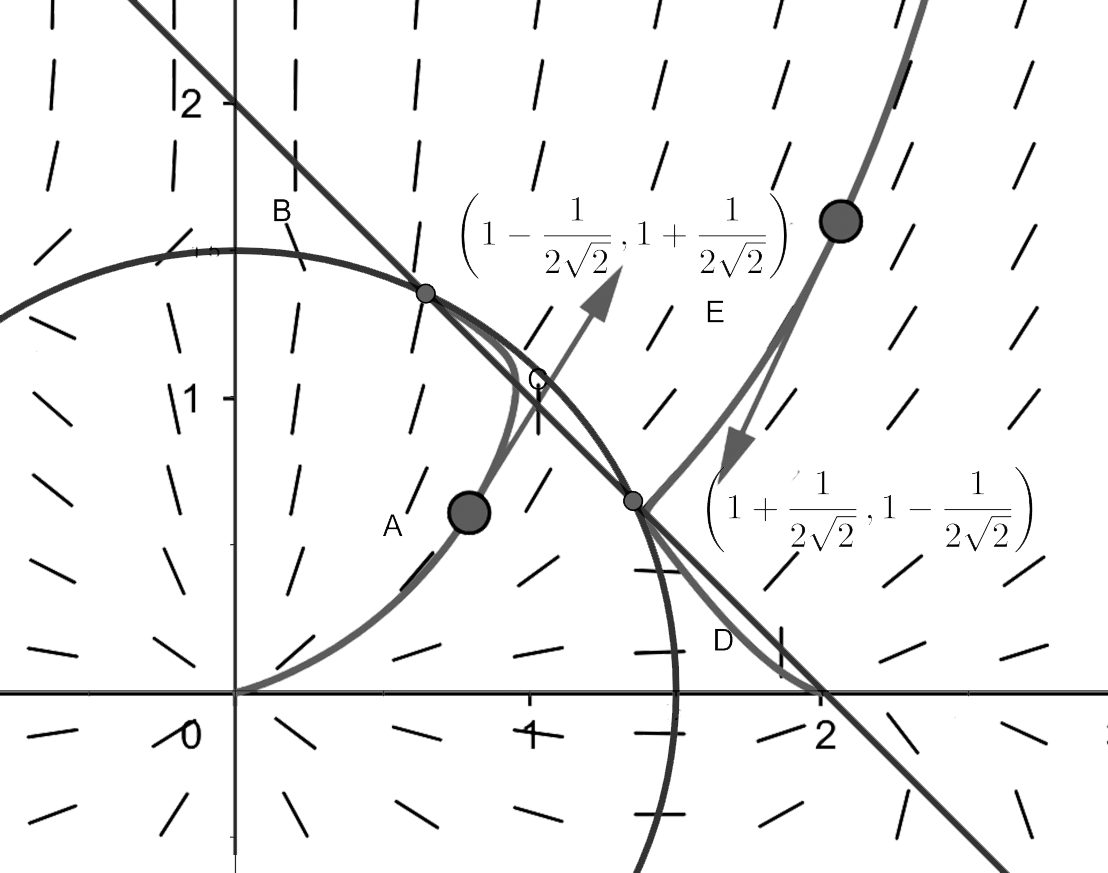
\includegraphics[width=12cm]{img/diam3-8_contodo.png}
\end{center}

c) Entonces tenemos los siguientes puntos críticos:
\[\begin{cases}
		\tex{Inestables: } (0,0), \left(1+\frac{1}{2\sqrt{2}}, 1-\frac{1}{2\sqrt{2}}\right), \left(0,\frac{3}{2}\right) \\
		\tex{Estables: } (2,0), \left(1-\frac{1}{2\sqrt{2}}, 1+\frac{1}{2\sqrt{2}}\right)
	\end{cases}\]
Calculamos la Jacobiana del sistema:
\[\operatorname{J}(k, d) = \begin{pmatrix}
		\pdv{k'}{k} & \pdv{k'}{d} \\
		\pdv{d'}{k} & \pdv{d'}{d}
	\end{pmatrix} = \begin{pmatrix}
		2-2k-d & -k                       \\
		-2kd   & \frac{9}{4} - 3d^2 - k^2
	\end{pmatrix}\]
\begin{enumerate}
	\item $\ds \operatorname{J}(2,0) = \begin{pmatrix}
			      -2 & -2           \\
			      0  & -\frac{7}{4}
		      \end{pmatrix} \implies \lambda_1, \lambda_2 < 0 \implies \tex{Estable}$
	\item $\ds \operatorname{J}\left(0, \frac{3}{2}\right) = \begin{pmatrix}
			      \frac{1}{2} & 0            \\
			      0           & -\frac{9}{2}
		      \end{pmatrix} \implies \lambda_1 = \frac{1}{2} \we \lambda_2 = -\frac{9}{2} \implies \tex{Inestable}$
\end{enumerate}

e) Queremos $\left(k(t_0), d(t_0)\right)$ tal que los dodos y los kiwis no se extinguen.

Si $\left(k(t_0), d(t_0)\right) \in C \ve B$, entonces no pueden escapar$\implies$ coexisten para siempre.

Si el punto inicial está en $D \implies$ Los dodos tienden a extinguirse.

Pero si el punto inicial está en $A$ se requiere un análisis más detallado.

f) En la región $E$ tenemos:$\ds k^2 + d^2 > \frac{9}{4} \we k+2 > 2 \implies k' < 0 \we d' > 0$.
\[\forall (k, d) \in E : V(k, d) \defeq k^2 + d^2 \implies \odv{}{t}V(k, d) = 2k k' + 2d d' < 0\]
\[\implies \forall t \in \R : k^2(t) + d^2(t) < k^2(t_0) + d^2(t_0) = C\]
Por tanto, $k^2+d^2$ es una cantidad disipativa y tenemos existencia global.